\documentclass[conference]{IEEEtran}
\IEEEoverridecommandlockouts
% The preceding line is only needed to identify funding in the first footnote. If that is unneeded, please comment it out.
\usepackage{cite}
\usepackage{amsmath,amssymb,amsfonts}
\usepackage{algorithmic}
\usepackage{graphicx}
\usepackage{textcomp}
\usepackage{xcolor}

\usepackage{multirow}


\def\BibTeX{{\rm B\kern-.05em{\sc i\kern-.025em b}\kern-.08em
    T\kern-.1667em\lower.7ex\hbox{E}\kern-.125emX}}
\begin{document}

\title{Estimate Power generation of invisible solar site using State estimation\\
% {\footnotesize \textsuperscript{*}Note: Sub-titles are not captured in Xplore and
% should not be used}
\thanks{PEA, AIT, NEU}
}

\author{\IEEEauthorblockN{1\textsuperscript{st} Pornchai Chaweewat}
\IEEEauthorblockA{\textit{EECC} \\
\textit{AIT)}\\
Pathumthani, Thailand \\
chaweewat.p@gmail.com}
\and
\IEEEauthorblockN{2\textsuperscript{nd} Weerakorn Ongsakul}
\IEEEauthorblockA{\textit{EECC} \\
\textit{AIT)}\\
Pathumthani, Thailand \\
email address}
\and
\IEEEauthorblockN{3\textsuperscript{rd} Jai Govind Singh}
\IEEEauthorblockA{\textit{EECC} \\
\textit{AIT)}\\
Pathumthani, Thailand \\
email address}
\and
\IEEEauthorblockN{4\textsuperscript{th} Ali abur}
\IEEEauthorblockA{\textit{EEC} \\
\textit{NEU}\\
Boston, MA, USA \\
email address}
}

\maketitle

\begin{abstract}
% This document is a model and instructions for \LaTeX.
% This and the IEEEtran.cls file define the components of your paper [title, text, heads, etc.]. *CRITICAL: Do Not Use Symbols, Special Characters, Footnotes,
% or Math in Paper Title or Abstract.
\end{abstract}

\begin{IEEEkeywords}
\end{IEEEkeywords}

\section{Introduction}


Sixty years ago, the price of solar panels was astronomical.  The price was over 1,000 US dollars per watt in today's money with 1 percent efficiency~\cite{b18}.
As the cost continues to drop, solar panel systems are becoming much more viable for the average household.
Today's price is less than 2.8 US dollars per watt for solar panel system including solar module, inverter, wiring hardware, labor cost, and maintenance cost~\cite{b19}.
As result of exponentially acceralate increasing in number of globally solar PV integration, especailly in residential sector.


Many researchers have studied the impacts and risks of PV on distribution systems \cite{b20}-~\cite{b25}.
However, the detection and monitoring of residential PV systems has not been the focus of the studies and related research.

Recently, the highest penetration of solar PV, recognized a large number of unauthorized solar PV installation \cite{b26}.
Unauthorized solar PV installation creates safety risks and lack of visibility may result in incorrect planning, and operation, including over-voltage, back-feeding.
Futhermore, in worst case scenario, it may damange system equipment such as transformers, voltage regulators, as well as customer applicants \cite{b15}, \cite{b16}.
In previous studies, there are various reasons for unauthorized or incorrectly registered PV system:
a) owner decided not to apply for a permit to avoid fees \cite{b17},
b) regulations were required after the system was installed,
c) lack of awareness by the owner of diverse permitting rules,
d) difference rules depending on size and type of PV installation can make the owners believe they do not need a permit
e) change in property ownership including transfer,
f) multiple system installed or future iaddition at the same premise,
g) incorrect third party handling of the permit appication,
h) data entry and data maintenance errors.





The rest of the paper is structured as follows: Section II reviews related research on state estimation application for power system and previous detection and estimation techniques on invisible solar PV site.
Section III formulates the mathenatic model of measurement data as well as the structure of proposed method.
Section IV shows the results of proposed method on test cases.
Section V conclueds the paper and dicusses future research oppotunities on PV system detection and estimation.


\section{Literature reviews}
%-----use of SE in power system

\section{Problem Formulation}

\begin{figure}[h!]
  \center
  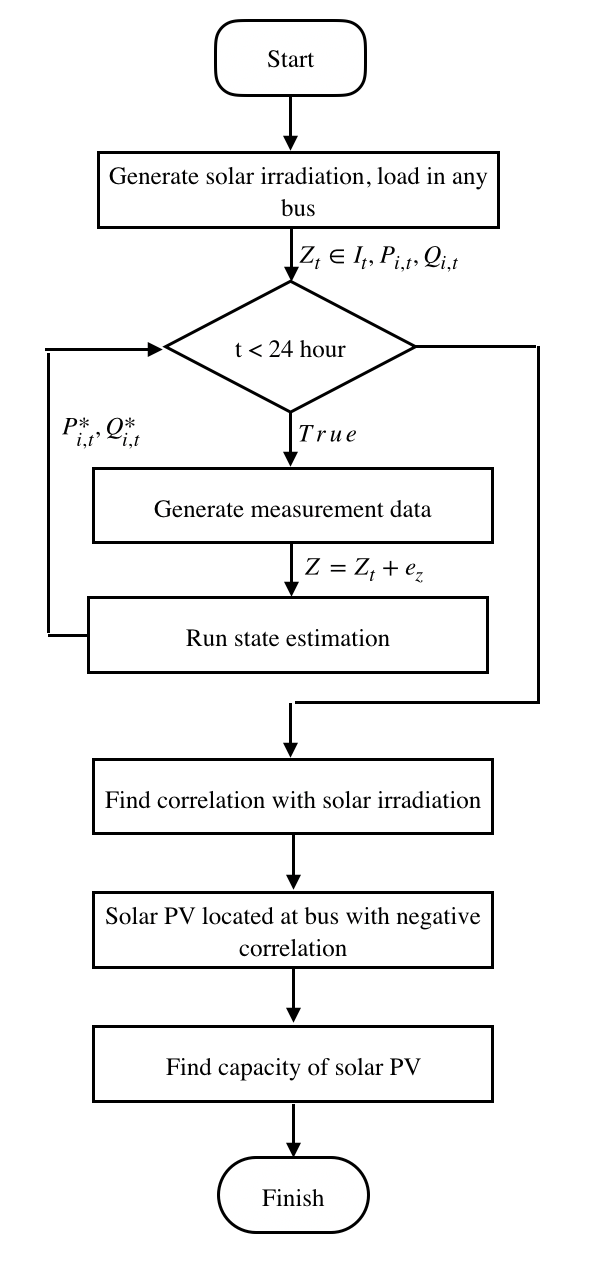
\includegraphics[scale=0.25]{images/conceptual_methodology.png}
  \caption{conceptual methodology}
  \label{fig.method}
\end{figure}

\subsection{Measurement devices, measured data and accuracy}

To generate measurement data for testing prurposes, measurement error was added to tha actual measurements as shown in Equation~\ref{eq.Z}.
\begin{equation}
  Z=Z_{a} \pm +e_{z}
\label{eq.Z}
\end{equation}
where $Z_{a}$ is actual data and $e_{z}$ is error added base on accuarcy of the measurement.
In this study, bus measurement has 3$\%$ error. line measurement has 5$\%$ error.

These error are assumed to be modeled independent Gaussian random variable\cite{b2}.
where where the error value is expected value from gaussian distribution.
noise is guassian distribution,as shown in Equation~\ref{eq.gaussian}
\begin{equation}
  g(x)=\frac{1}{\sigma \sqrt{2\pi}}e^{-\frac{1}{2}((x-\mu)/\sigma)^2}
  \label{eq.gaussian}
\end{equation}
\subsubsection{State variable description:} voltage, current, power flow from measurements devices

\subsection{Peform SE to find }
\subsubsection{LWS}
\subsubsection{Branch current, load allocation based state estimation}
is based on the weighted least square (WLS) approach\cite{b1}.
the method solves the following WLS problem to obtain an estimate ofthe system operating point defined by the system state x:
\begin{equation}
  \underset{x}{min} J(x)=\sum_{i=1}^{m}w_{i}(z_{i}-h_{i}(x))^{2}=\big[ z-h(x)\big]^{T}W\big[z-h(x)\big]
\label{eq.jacobian}
\end{equation}
where $w_{i}$ and $h_{i}(x)$ represent the weight and the measurements function associated with measurement $z_{i}$, respectively.
For the solution of this problem the conventional iterative method is adape by solving following normal equations at each iteration, to compute the update $x^{k+1}=x^{k}+\Delta x^{k}$
\begin{equation}
  \big[G(x^{k})\big]\Delta x^{k} = H^{T}(x^{k})W \big[ z-h(x^{k}) \big]
  \label(eq.delta_x)
\end{equation}

Where

\begin{equation}
  G(x)=H^{T}(x)WH(x)
  \label(eq.gain)
\end{equation}

is the gain matrix and H is the jacobian of the measurement function $h(x)$.

\subsection{Find correlation with solar irradiation}

A correlation is a statistical measure of relationship between two variables. The measure is best used in variables that demenstrate a linear relationship between each other.
The correlation coefficient that indicates the straength of the relationship between two variables can be found using following formula:

\begin{equation}
  \text{r}_{xy} =\frac{\sum(x_{i}-\overline{x})(y_{i}-\overline{y})}{\sqrt{\sum(x_{i}-\overline{y})^{2}(y_{i}-\overline{y})^{2})}}
  \label{eq.corr}
\end{equation}

where $\text{r}_{xy}$ is the correlation coefficient of the linear relationship between the variables x and y, $x_{i}$ is the values of the x-variable in a sample, $\overline{x}$ is the mean of the varialbes of the x-variable,
$y_{i}$ is the values of the y-variable in a sample, $\overline{y}$ is the mean of the varialbes of the y-variable.

The negaive correlation shows that the variables tend to move in opposity directions (i.e., when one variable increases, the other variable decreases).

\subsection{Find capacity of solar PV using changing point method}


\section{Test Cases and Results}


\section{Conclusion}
Here is Conclusion.



\section*{Acknowledgment}

\begin{thebibliography}{00}
  \bibitem{b18} https://www.theguardian.com/sustainable-business/2016/jan/31/solar-power-what-is-holding-back-growth-clean-energy
  \bibitem{b19} https://blog.pickmysolar.com/the-price-of-a-solar-panel-system-over-the-years
  \bibitem{b20} M. E. Baran, H. Hooshyar, Z. Shen, and A. Huang, “Accommodating high PV penetration on distribution feeders,” IEEE Trans. Smart Grid, vol. 3, no. 2, pp. 1039–1046, Jun. 2012.
  \bibitem{b21}  M. J. Reno, K. Coogan, R. J. Broderick, J. Seuss, and S. Grijalva, “Impact of PV variability and ramping events on distribution voltage regulation equipment,” in Proc. IEEE Photovolt. Spec. Conf., Tampa, FL, USA, 2014.
  \bibitem{b22} M. E. Baran, H. Hooshyar, Z. Shen, and A. Huang, “Accommodating high PV penetration on distribution feeders,” IEEE Trans. Smart Grid, vol. 3, no. 2, pp. 1039–1046, Jun. 2012.
  \bibitem{b23} P. Li, X. Yu, J. Zhang, and Z. Yin, “The H∞ control method of grid- tied photovoltaic generation,” IEEE Trans. Smart Grid, vol. 6, no. 4, pp. 1670–1677, Jul. 2015.
  \bibitem{b24}  A. Samadi, L. Söder, E. Shayesteh, and R. Eriksson, “Static equivalent of distribution grids with high penetration of PV systems,” IEEE Trans. Smart Grid, vol. 6, no. 4, pp. 1763–1774, Jul. 2015.
  \bibitem{b25}  H. Ravindra et al.,“Impact of PV on distribution protection system,” in Proc. North Amer. Power Symp. (NAPS), Champaign, IL, USA, Sep. 2012, pp. 1–6.
  \bibitem{b26} P. Fairley. (Jan. 2015). Hawaii’ s Solar Push Strains the Grid. [online]. Available: http://www.technologyreview.com/news/534266/ hawaiis-solar-push-strains-the-grid/
  \bibitem{b15} W. Staff. (Sep. 2014). Heco Customers Asked to Disconnect Unauthorized PV Systems. [Online]. Available: http://khon2.com/2014/ 09/05/heco-customers-asked-to-disconnect-unauthorized-pv-systems/
  \bibitem{b16} V. Schwarzer and R. Ghorbani, “Transient over-voltage mitiga- tion: Explanation and mitigation options for inverter-based dis- tributed generation projects,” Elect.Vehicle Transp. Center, Sch. Ocean Earth Sci. Technol., Univ. Hawai’ i Manoa, Honolulu, HI, US A , Tech. Rep. HNEI-02-15, Feb. 2014.
  \bibitem{b17} https://www.snopes.com/fact-check/is-it-illegal-florida-power-home-solar-storm/
  \bibitem{b1} Roytelman I. and S.M. Shahidehpour, ‘State estimation for electric power distribution systems in quasi real-time conditions’, IEEE Trans. Power Systems, 1993 winter meeting, paper no:090-1-PW RD.
  \bibitem{b2} A. Abur and A. G. Exposito, Power System State Estimation: Theory and Implementation. New York: Marcel Dekker, 2004.
  \bibitem{b3} CIGRE' Task Force C6.04.02: Developing benchmark models for integrating distributed energy resourcesS. Barsali, Kai Strunz, Zbigniew StyczynskiPublished 2005
  \bibitem{b4} STATE ESTIMATION FOR LOAD ALLOCATION IN DISTRIBUTION POWER SYSTEMS, R. Sharifian 1 E. Jafari 1 M. Rahimi 2 P. Ghaebi Panah 3
  \bibitem{b5} A Revised Branch Current-Based Distribution System State Estimation Algorithm and Meter Placement Impact, Haibin Wang, Student Member, IEEE, and Noel N. Schulz, Senior Member, IEEE
  \bibitem{b6} An Integrated Load AllocatiodState Estimation Approach for Distribution Networks, JorgePereira, J. T. Saraiva,Member, IEEE, V. Miranda, Member, IEEE
  \bibitem{b7} Distribution System State Estimation Using AMI Data, Mesut Baran, T. E. McDermott
  \bibitem{b8} Gu Chaojun, Student Member, IEEE, Panida Jirutitijaroen, Senior Member, IEEE, and Mehul Motani, Member, IEEE, Detecting False Data Injection Attacks in AC State Estimation
  \bibitem{b9} A Review on Distribution System State Estimation, Anggoro Primadianto and Chan-Nan Lu, Fellow, IEEE
  \bibitem{b10} Nathan Wallace, Stanislav Ponomarev, and Travis Atkison, Identification of Compromised Power System State Variables
  \bibitem{b11} X. Zhang and S. Grijalva, “A data-driven approach for detection and estimation of residential pv installations,” IEEE Transactions on Smart Grid, vol. 7, no. 5, pp. 2477–2485, Sept 2016.
  \bibitem{b12} H. Shaker, H. Zareipour, and D. Wood, “Estimating power generation of invisible solar sites using publicly available data,” IEEE Transactions on Smart Grid, vol. 7, no. 5, pp. 2456–2465, Sept 2016.
  \bibitem{b13} H. Jiang, X. Dai, D. W. Gao, J. J. Zhang, Y. Zhang, and E. Muljadi, “Spatial-temporal synchrophasor data characterization and analytics in smart grid fault detec- tion, identification, and impact causal analysis,” IEEE Transactions on Smart Grid, vol. 7, no. 5, pp. 2525– 2536, Sept 2016.
  \bibitem{b14} Detection and Estimation of the Invisible Units Using Utility Data Based on Random Matrix Theory, Xing He, Robert C. Qiu, Fellow, IEEE, Lei Chu, Qian Ai, Zenan Ling, Jian Zhang
\end{thebibliography}

% \section*{References}
%
% \begin{thebibliography}{00}
% \end{thebibliography}


% \section{Introduction}
% This document is a model and instructions for \LaTeX.
% Please observe the conference page limits.
%
% \section{Ease of Use}
%
% \subsection{Maintaining the Integrity of the Specifications}
%
% The IEEEtran class file is used to format your paper and style the text. All margins,
% column widths, line spaces, and text fonts are prescribed; please do not
% alter them. You may note peculiarities. For example, the head margin
% measures proportionately more than is customary. This measurement
% and others are deliberate, using specifications that anticipate your paper
% as one part of the entire proceedings, and not as an independent document.
% Please do not revise any of the current designations.
%
% \section{Prepare Your Paper Before Styling}
% Before you begin to format your paper, first write and save the content as a
% separate text file. Complete all content and organizational editing before
% formatting. Please note sections \ref{AA}--\ref{SCM} below for more information on
% proofreading, spelling and grammar.
%
% Keep your text and graphic files separate until after the text has been
% formatted and styled. Do not number text heads---{\LaTeX} will do that
% for you.
%
% \subsection{Abbreviations and Acronyms}\label{AA}
% Define abbreviations and acronyms the first time they are used in the text,
% even after they have been defined in the abstract. Abbreviations such as
% IEEE, SI, MKS, CGS, ac, dc, and rms do not have to be defined. Do not use
% abbreviations in the title or heads unless they are unavoidable.
%
% \subsection{Units}
% \begin{itemize}
% \item Use either SI (MKS) or CGS as primary units. (SI units are encouraged.) English units may be used as secondary units (in parentheses). An exception would be the use of English units as identifiers in trade, such as ``3.5-inch disk drive''.
% \item Avoid combining SI and CGS units, such as current in amperes and magnetic field in oersteds. This often leads to confusion because equations do not balance dimensionally. If you must use mixed units, clearly state the units for each quantity that you use in an equation.
% \item Do not mix complete spellings and abbreviations of units: ``Wb/m\textsuperscript{2}'' or ``webers per square meter'', not ``webers/m\textsuperscript{2}''. Spell out units when they appear in text: ``. . . a few henries'', not ``. . . a few H''.
% \item Use a zero before decimal points: ``0.25'', not ``.25''. Use ``cm\textsuperscript{3}'', not ``cc''.)
% \end{itemize}
%
% \subsection{Equations}
% Number equations consecutively. To make your
% equations more compact, you may use the solidus (~/~), the exp function, or
% appropriate exponents. Italicize Roman symbols for quantities and variables,
% but not Greek symbols. Use a long dash rather than a hyphen for a minus
% sign. Punctuate equations with commas or periods when they are part of a
% sentence, as in:
% \begin{equation}
% a+b=\gamma\label{eq}
% \end{equation}
%
% Be sure that the
% symbols in your equation have been defined before or immediately following
% the equation. Use ``\eqref{eq}'', not ``Eq.~\eqref{eq}'' or ``equation \eqref{eq}'', except at
% the beginning of a sentence: ``Equation \eqref{eq} is . . .''
%
% \subsection{\LaTeX-Specific Advice}
%
% Please use ``soft'' (e.g., \verb|\eqref{Eq}|) cross references instead
% of ``hard'' references (e.g., \verb|(1)|). That will make it possible
% to combine sections, add equations, or change the order of figures or
% citations without having to go through the file line by line.
%
% Please don't use the \verb|{eqnarray}| equation environment. Use
% \verb|{align}| or \verb|{IEEEeqnarray}| instead. The \verb|{eqnarray}|
% environment leaves unsightly spaces around relation symbols.
%
% Please note that the \verb|{subequations}| environment in {\LaTeX}
% will increment the main equation counter even when there are no
% equation numbers displayed. If you forget that, you might write an
% article in which the equation numbers skip from (17) to (20), causing
% the copy editors to wonder if you've discovered a new method of
% counting.
%
% {\BibTeX} does not work by magic. It doesn't get the bibliographic
% data from thin air but from .bib files. If you use {\BibTeX} to produce a
% bibliography you must send the .bib files.
%
% {\LaTeX} can't read your mind. If you assign the same label to a
% subsubsection and a table, you might find that Table I has been cross
% referenced as Table IV-B3.
%
% {\LaTeX} does not have precognitive abilities. If you put a
% \verb|\label| command before the command that updates the counter it's
% supposed to be using, the label will pick up the last counter to be
% cross referenced instead. In particular, a \verb|\label| command
% should not go before the caption of a figure or a table.
%
% Do not use \verb|\nonumber| inside the \verb|{array}| environment. It
% will not stop equation numbers inside \verb|{array}| (there won't be
% any anyway) and it might stop a wanted equation number in the
% surrounding equation.
%
% \subsection{Some Common Mistakes}\label{SCM}
% \begin{itemize}
% \item The word ``data'' is plural, not singular.
% \item The subscript for the permeability of vacuum $\mu_{0}$, and other common scientific constants, is zero with subscript formatting, not a lowercase letter ``o''.
% \item In American English, commas, semicolons, periods, question and exclamation marks are located within quotation marks only when a complete thought or name is cited, such as a title or full quotation. When quotation marks are used, instead of a bold or italic typeface, to highlight a word or phrase, punctuation should appear outside of the quotation marks. A parenthetical phrase or statement at the end of a sentence is punctuated outside of the closing parenthesis (like this). (A parenthetical sentence is punctuated within the parentheses.)
% \item A graph within a graph is an ``inset'', not an ``insert''. The word alternatively is preferred to the word ``alternately'' (unless you really mean something that alternates).
% \item Do not use the word ``essentially'' to mean ``approximately'' or ``effectively''.
% \item In your paper title, if the words ``that uses'' can accurately replace the word ``using'', capitalize the ``u''; if not, keep using lower-cased.
% \item Be aware of the different meanings of the homophones ``affect'' and ``effect'', ``complement'' and ``compliment'', ``discreet'' and ``discrete'', ``principal'' and ``principle''.
% \item Do not confuse ``imply'' and ``infer''.
% \item The prefix ``non'' is not a word; it should be joined to the word it modifies, usually without a hyphen.
% \item There is no period after the ``et'' in the Latin abbreviation ``et al.''.
% \item The abbreviation ``i.e.'' means ``that is'', and the abbreviation ``e.g.'' means ``for example''.
% \end{itemize}
% An excellent style manual for science writers is \cite{b7}.
%
% \subsection{Authors and Affiliations}
% \textbf{The class file is designed for, but not limited to, six authors.} A
% minimum of one author is required for all conference articles. Author names
% should be listed starting from left to right and then moving down to the
% next line. This is the author sequence that will be used in future citations
% and by indexing services. Names should not be listed in columns nor group by
% affiliation. Please keep your affiliations as succinct as possible (for
% example, do not differentiate among departments of the same organization).
%
% \subsection{Identify the Headings}
% Headings, or heads, are organizational devices that guide the reader through
% your paper. There are two types: component heads and text heads.
%
% Component heads identify the different components of your paper and are not
% topically subordinate to each other. Examples include Acknowledgments and
% References and, for these, the correct style to use is ``Heading 5''. Use
% ``figure caption'' for your Figure captions, and ``table head'' for your
% table title. Run-in heads, such as ``Abstract'', will require you to apply a
% style (in this case, italic) in addition to the style provided by the drop
% down menu to differentiate the head from the text.
%
% Text heads organize the topics on a relational, hierarchical basis. For
% example, the paper title is the primary text head because all subsequent
% material relates and elaborates on this one topic. If there are two or more
% sub-topics, the next level head (uppercase Roman numerals) should be used
% and, conversely, if there are not at least two sub-topics, then no subheads
% should be introduced.
%
% \subsection{Figures and Tables}
% \paragraph{Positioning Figures and Tables} Place figures and tables at the top and
% bottom of columns. Avoid placing them in the middle of columns. Large
% figures and tables may span across both columns. Figure captions should be
% below the figures; table heads should appear above the tables. Insert
% figures and tables after they are cited in the text. Use the abbreviation
% ``Fig.~\ref{fig}'', even at the beginning of a sentence.
%
% \begin{table}[htbp]
% \caption{Table Type Styles}
% \begin{center}
% \begin{tabular}{|c|c|c|c|}
% \hline
% \textbf{Table}&\multicolumn{3}{|c|}{\textbf{Table Column Head}} \\
% \cline{2-4}
% \textbf{Head} & \textbf{\textit{Table column subhead}}& \textbf{\textit{Subhead}}& \textbf{\textit{Subhead}} \\
% \hline
% copy& More table copy$^{\mathrm{a}}$& &  \\
% \hline
% \multicolumn{4}{l}{$^{\mathrm{a}}$Sample of a Table footnote.}
% \end{tabular}
% \label{tab1}
% \end{center}
% \end{table}
%
% \begin{figure}[htbp]
% \centerline{\includegraphics{fig1.png}}
% \caption{Example of a figure caption.}
% \label{fig}
% \end{figure}
%
% Figure Labels: Use 8 point Times New Roman for Figure labels. Use words
% rather than symbols or abbreviations when writing Figure axis labels to
% avoid confusing the reader. As an example, write the quantity
% ``Magnetization'', or ``Magnetization, M'', not just ``M''. If including
% units in the label, present them within parentheses. Do not label axes only
% with units. In the example, write ``Magnetization (A/m)'' or ``Magnetization
% \{A[m(1)]\}'', not just ``A/m''. Do not label axes with a ratio of
% quantities and units. For example, write ``Temperature (K)'', not
% ``Temperature/K''.
%
% \section*{Acknowledgment}
%
% The preferred spelling of the word ``acknowledgment'' in America is without
% an ``e'' after the ``g''. Avoid the stilted expression ``one of us (R. B.
% G.) thanks $\ldots$''. Instead, try ``R. B. G. thanks$\ldots$''. Put sponsor
% acknowledgments in the unnumbered footnote on the first page.
%
% \section*{References}
%
% Please number citations consecutively within brackets \cite{b1}. The
% sentence punctuation follows the bracket \cite{b2}. Refer simply to the reference
% number, as in \cite{b3}---do not use ``Ref. \cite{b3}'' or ``reference \cite{b3}'' except at
% the beginning of a sentence: ``Reference \cite{b3} was the first $\ldots$''
%
% Number footnotes separately in superscripts. Place the actual footnote at
% the bottom of the column in which it was cited. Do not put footnotes in the
% abstract or reference list. Use letters for table footnotes.
%
% Unless there are six authors or more give all authors' names; do not use
% ``et al.''. Papers that have not been published, even if they have been
% submitted for publication, should be cited as ``unpublished'' \cite{b4}. Papers
% that have been accepted for publication should be cited as ``in press'' \cite{b5}.
% Capitalize only the first word in a paper title, except for proper nouns and
% element symbols.
%
% For papers published in translation journals, please give the English
% citation first, followed by the original foreign-language citation \cite{b6}.
%
% \begin{thebibliography}{00}
% \bibitem{b1} G. Eason, B. Noble, and I. N. Sneddon, ``On certain integrals of Lipschitz-Hankel type involving products of Bessel functions,'' Phil. Trans. Roy. Soc. London, vol. A247, pp. 529--551, April 1955.
% \bibitem{b2} J. Clerk Maxwell, A Treatise on Electricity and Magnetism, 3rd ed., vol. 2. Oxford: Clarendon, 1892, pp.68--73.
% \bibitem{b3} I. S. Jacobs and C. P. Bean, ``Fine particles, thin films and exchange anisotropy,'' in Magnetism, vol. III, G. T. Rado and H. Suhl, Eds. New York: Academic, 1963, pp. 271--350.
% \bibitem{b4} K. Elissa, ``Title of paper if known,'' unpublished.
% \bibitem{b5} R. Nicole, ``Title of paper with only first word capitalized,'' J. Name Stand. Abbrev., in press.
% \bibitem{b6} Y. Yorozu, M. Hirano, K. Oka, and Y. Tagawa, ``Electron spectroscopy studies on magneto-optical media and plastic substrate interface,'' IEEE Transl. J. Magn. Japan, vol. 2, pp. 740--741, August 1987 [Digests 9th Annual Conf. Magnetics Japan, p. 301, 1982].
% \bibitem{b7} M. Young, The Technical Writer's Handbook. Mill Valley, CA: University Science, 1989.
% \end{thebibliography}
% \vspace{12pt}
% \color{red}
% IEEE conference templates contain guidance text for composing and formatting conference papers. Please ensure that all template text is removed from your conference paper prior to submission to the conference. Failure to remove the template text from your paper may result in your paper not being published.

\end{document}
